\documentclass[a4paper, 12pt]{article}

\usepackage[english]{babel}
\usepackage[utf8]{inputenc}
\usepackage [autostyle, english = american]{csquotes}
\MakeOuterQuote{"}
\usepackage{url}
\usepackage{import}
\usepackage{tabularx}
\usepackage{booktabs}
\usepackage{amsmath}
\usepackage{amsfonts}
\usepackage{graphicx}
\usepackage[margin=1.25in]{geometry}
\usepackage{caption}
\usepackage{multirow}
\usepackage[table]{xcolor}
\usepackage{rotating}
\usepackage{mathtools}
\usepackage[multiple]{footmisc}
\usepackage{xr}
\usepackage{breakcites}
\usepackage{matlab-prettifier}
\usepackage[]{mcode}
\usepackage{listings}
\usepackage{color}
\usepackage{hyperref}
\usepackage{authblk}

\title {Profile Ranking Adaptive Choice-Based Conjoint Analysis: A Complementary Approach to Utility-Based Analysis for Small Populations}

 \author[1]{}
% \author[1]{Skyler Laney\thanks{skyler.laney@my.wheaton.edu}}

% \author[1]{Leo O'Malley\thanks{leo.omalley@my.wheaton.edu}}
% \author[1]{Cathy Shi\thanks{cathy.shi@my.wheaton.edu}}
% \author[1]{Danilo Diedrichs\thanks{danilo.diedrichs@wheaton.edu}}
% \author[1]{Nate Schatz\thanks{Nate.Schatz@my.wheaton.edu}
% \affil[1]{Department of Mathematics, Wheaton College}
\date{}

\usepackage[]{mcode}
\usepackage{matlab-prettifier}
\usepackage{listings} %For code in appendix
\usepackage{color} %red, green, blue, yellow, cyan, magenta, black, white
\definecolor{mygreen}{RGB}{28,172,0} % color values Red, Green, Blue
\definecolor{mylilas}{RGB}{170,55,241}
\usepackage{gensymb}
\usepackage{makeidx}
\makeindex
\pagestyle{empty}
\usepackage{endnotes}
\usepackage{lineno}
%\linenumbers
\begin{document}

%%%%For color MATLAB Scripts
\lstset
{ %Formatting for code in appendix
    language=Matlab,
    basicstyle=\scriptsize,
    numbers=left,
    stepnumber=1,
    showstringspaces=false,
    tabsize=1,
    breaklines=true,
    breakatwhitespace=false,
}
\maketitle
\hrulefill
\externaldocument{targettable}
\externaldocument{SimpleEquityModel}

 \vspace{.7in}

 \begin{abstract}
To analyze Adaptive Choice-Based Conjoint (ACBC) survey samples from small populations, a new methodology called profile ranking based ACBC (PR-ACBC) is proposed as a complement to utility based  ACBC. PR-ACBC offers a form of validation especially useful for small survey data with high variances in partworth utilities. Without requiring knowledge of partworth utilities, PR-ACBC begins with a simple computation using choice task data to obtain both individual and sample mean profile attribute level (PAL) rankings. the Maximum likelihood estimation of profile rankings for both known population size $N$ (multivariate hypergeometric distribution) and unkown $N$ (Lagrange multiplier optimization) is then used to obtain point estimates of population PALs. A PAL ranking interval can easily be computed  for each level as an interval guaranteed to include  each PAL for any specified vale of $N$. The sample PAL rankings are also used  for  multidimensional scaling (MDS) which offers a two-dimensional visual representation of similarities/dissimilarities in respondents or PALs.  Attribute level rankings are then compared with partworth utilities with respect to accuracy of choice task predictions and ranking of attribute importances. Finally, PR-ACBC methodology is applied to a recent survey administered to  a small population of disaster relief organizations belonging to the National Voluntary Organizations Active in Disaster (VOAD).

\end{abstract}

%% THIS IS FOR A SHORT SCRIPT

% \begin{table}[!htpb]
%  \begin{tabular}{|l|}\toprule
%  {\bf MATLABScript.m}\\\hline
%  \parbox[b]{5.75in}{\lstinputlisting[style=Matlab-editor]{MATLABScript.m}}\\\hline\hline
%  \bottomrule
%  \end{tabular}
%  \end{table}

%% THIS IS FOR A LONG SCRIPT WHICH MUST BE SPLIT INTO
%% SHORTER BLOCK OF CODE YOU CAN SPECIFY THE
%% RANGE OF LINE NUMBERS DISPLAYED AND NUMBER
%% OF THE FIRST LINE

%  \begin{table}[!htpb]
% \centering
% \begin{tabular}{|l|}\hline
% MATLABScript.m. (p1 of 1)\\\hline
% \parbox[b]{5.8in}{\lstinputlisting[style=Matlab-editor,firstline=20, lastline=32, firstnumber=20]{MATLABScript.m}}\\\hline
% \end{tabular}
% \end{table}

 \vspace{1in}

\section{Introduction}

Adaptive Choice-Based Conjoint (ACBC) analysis surveys are a widely-utilized, well-developed, and highly effective  type of conjoint analysis (Orme and Chrzan, 2017). While the Max-Diff approach to select the best and worst among several profiles in a choice task has generated a great deal of recent interest, we focus on ACBC surveys whose choice tasks are designed with the  simplest choice between just two concepts. Based on our experience with small population  (eg. $N\le 50$) nationwide on-line surveys we created using Sawtooth's Lighthouse platform, we structure our choice-task stage as a single-elimination tournament beginning with a small number of profiles close to the respondent's \#1 profile revealed in the  ``Build Your Own'' (BYO) stage. For large samples, use of a sophisticated statistical method such as hierarchical-Bayesian Markov-Chain Monte-Carlo (HB MCMC) simulation (Rossi et. al. 2005) is extremely effective to estimate partworth utilities and their variances. In the case of small samples  (eg. $n \le$ 15) from a small population, large variances in partworth utilities may hamper both accurate prediction of choice experiments  and ranking of attribute importances.  Profile attribute rankings (PARs) which can easily be computed without utilities serve as a validity check for profile choice predictions and attribute importances based on part-worth utilities.  PARs are also used in  multi-dimensional scaling (MDS) (Alvo and Yu 2014) to give a 2-dimensional visual representation showing similarities in respondents and their ranking of attribute levels.

In Section 2, we introduce basic PR-ACBC methodology by means of a very simple generic survey with only 4 profiles constructed from 2 attributes each with 2 levels. We begin with a fundamental observation that the exact sample profile rankings directly obtainable from choice tournament data can not be obtained by multiple linear regression (part-worth utilities).  PR-ACBC then proceeds to analyze  survey tournament data without requiring any knowledge of partworth utilities.  Maximum likelihood estimate (MLE) population rankings for known population sizes are obtainable by a discrete multivariate hypergeometric distribution (Oberhofer and Kaufman 1987), and  for unknown population sizes by multivariable calculus optimization using Lagrange multipliers (Stewart 2016).   Population ranking intervals (PRIs) which must contain the unkown population profile rankings are easily computed from sample profile rankings.Similarly, the PAR-intervals which must contain the actual population attribute level rankings are easily obtained from sample data.   Sample PARs are also useful for multi-dimensional scaling (MDS) which show similarities in respondents and PAL rankings. This is useful for comparing and contrasting sample subgroups.  In Section 3 we illustrate PR methodology using a recent ACBC survey deployed to both faith-based and non-faith based disaster relief organizations.    The context motivating this methodological study is a sequel to a novel application of ACBC in disaster-response research (Gralla et. al. 2014).



\section{PR-ACBC Methodology}
In this section we introduce PR-ACBC methodology using a simple example.

\subsection{Simple Example}

Consider a generic ``toy'' ACBC survey with just 2 attributes each having 2 levels. We designate the 4 possible profiles $A=11, B=10, C=01, D=00$, where $X=x_1x_2$ designates that profile $X$ has level $x_1$ for the first attribute and level $x_2$ for the second attribute. Suppose we have obtained by anonymous survey choice tournament results  for $n=4$ respondents from a population of size $N>4$.  A sample tournament outcome is shown in Figure \ref{SimpleTourn}
\begin{figure}[!htpb]
\centering
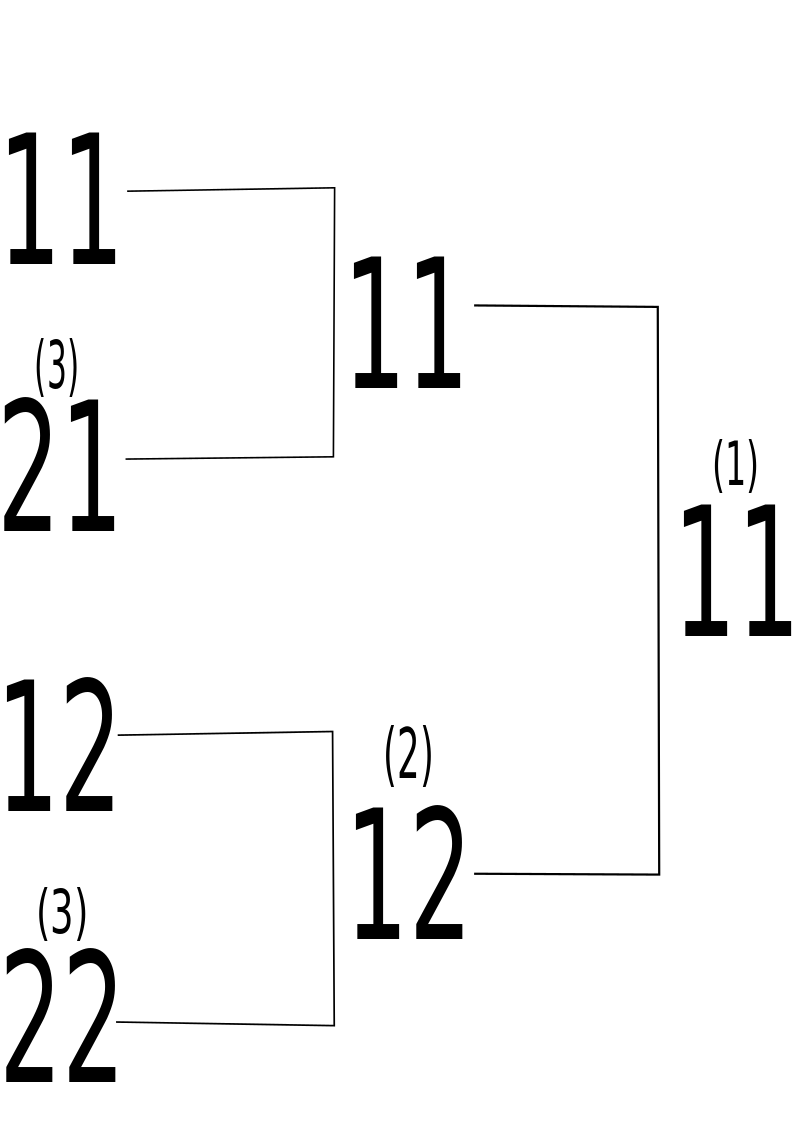
\includegraphics[width=1.75in, height=1.5in]{SimpleTourn.png}
\caption{A respondent whose tournament data ranks profile A=11 first, C=01 second, B=10 is ranked third and D=00 fourth.  }
\label{SimpleTourn}
\end{figure}

{\flushleft This} respondent profile ranking is denoted ACBD, meaning profile A=11 is ranked 1 (tournament winner), profile C=01 is ranked 2 (runner-up), profile B=10 third, and D=00 ranked 4th. The rationale for the latter 2 rankings is that assuming transitivity in match outcomes, the highest B could be ranked if all profiles were paired is 2, while D could only be ranked as high as 3. 

In our toy survey with just 4 possible profiles, there are already 4!=24 possible profile rankings. In the next section we consider an actual survey of disaster relief organizations (DROs) with 4 attributes containing 3 levels each, administered to a population of roughly $N=50$ faith based disaster relief organizations. This survey  has 81 profiles and 81!=5 797 126 020 747 367 985 879 734 231 578 109 105 412 357 244 731 625 958 745 865 049 716 390
 179 693 892 056 256 184 534 249 745 940 480 000 000 000 000 000 000 profile rankings,  For a sample size of $n=13$, and a choice task stage  which provides each respondent's ranking of 16 profiles, a meaningful ranking of  all the profiles is evidently impossible. As a result, our approach to ranking profiles, one more akin to using partworth utilities to determine profile choices, is to rank individual attribute levels rather than profiles as a whole. 

Our toy survey has just four profile levels which we denote $(x_1,x_2)$ where $x_1$ is the attribute number (1 or 2) and $x_2$ the level number (0 or 1). Note that each level appears in exactly two profiles. For each attribute level, we compute a respondent's profile attribute level (PAL) ranking as the average of the two profile rankings in which the level appears.  For example since $(1,0)$ appears in profiles $C$ and $D$, if a respondent's profile ranking is ACBD, then the $(1,0)$ PAL ranking is (2+4)/2=3. (See Table \ref{PAL1})


\begin{table}[!htpb]
	
	\centering
	\begin{tabular}{c|cccc}
		Profile&\multicolumn{4}{c}{PAL Ranking}\\
		Ranking&(1,1)&(1,0)&(2,1),&(2,0)\\\hline
		ABCD& 1.5&3.5&2&3\\
		ACBD& 2&3&1.5&3.5\\
		BADC&1.5&3.5&3&2 \\
		CBAD& 2.5&2.5&2&3 \\\hline
		$m$&1.875&3.375&2.125&2.875\\
		$s$ &.4787&.25&.6292&.6292\\
	\end{tabular}
	\caption{Example of sample PAL rankings ($n=4$, $m$=mean, $s$=standard deviation, profiles A=11,B=10,C=01, and D=00.)}
	\label{PAL1}
\end{table}



In our DRO survey, there are  a total of 12 PALs $(x_1,x_2)$ with $x_1\in\{1,2,3,4\}$ and $x_2\in\{1,2,3\}$. Each PAL occurs in 27 out of the 81 profiles and has roughly a 99.85\% chance of appearing in a  in a single elimination round of 16 tournament (and hence have a ranking between 1 and 16). PALs not appearing in a tournament are assigned a ranking of 24.5 (the average of rankings 17 through 32 which would be assigned to the first round losers had one earlier round been included in the tournament.)  In short, PAL rankings are far more meaningful than profile rankings.



The main questions we will develop in the sequel are: 
\begin{itemize}
\item POPULATION INFERENCES: \emph{what can we infer from sample PAL rankings about the population PAL rankings?}; and
\item APPLICATION TO REAL SURVEYS:  \emph{How well do PAL rankings predict  choice-tasks and attribute importances in the DRO survey?}
\end{itemize}

\subsection{A Fundamental Observation}
In this section we show that  least squares multiple  regression (LSRM) will not in general give exact sample profile rankings and their corresponding PAL rankings. In other words, part-worth utilities can only approximate sample PAL rankings.


Least squares multiple linear regression (LSRM) can be used to predict sample PAL rankings as we will now explain using our toy survey.  Let $U$ denote the level of attribute 1, $V$ the level of attribute 2, and $Y$ the ranking of a profilw with levels $U$ and $V$. Table \ref{Tab7} gives the dataset \{($U_i,V_i,Y_i$)\} ($i = 1,...,16$) where

\begin{eqnarray*}
	U_i&=& 1 \textup{ if attribute 1 has level 1, and 0 if it has level 2}\\
	V_i&=& 1 \textup{ if attribute 2 has level 1, and 0 if it has level 2}\\
	Y_i&=& \textup{ Respondent's ranking of a profile with $U=U_i$, $V=V_i$.}
\end{eqnarray*}

\begin{table}[!htpb]
	\centering
	\small
	\begin{tabular}{cc|ccccc}	\hline
		$U$ & $V$ & Respondent 1&  Respondent 2& Respondent 3& Respondent 4\\  \hline
		1 &1&$Y_1$&$Y_2$&$Y_3$&$Y_4$\\
		1 &0&$Y_5$&$Y_6$&$Y_7$&$Y_8$ \\
		0 &1&$Y_9$&$Y_{10}$&$Y_{11}$&$Y_{12}$ \\
		0 &0&$Y_{13}$&$Y_{14}$&$Y_{15}$&$Y_{16}$ \\\hline
	\end{tabular}
	\caption{{\small Sample profile rankings by respondent ($n=4$).}}
	\label{Tab7}
\end{table}


This dataset has certain properties:
\begin{itemize}
	\item
	Each column consists of a respondent's profile rankings and so contains the numbers 1,2,3 and 4.
	\item
	Table \ref{Tab7} can also be represented in the form of Table \ref{Tab8}, by which we see that $$\sum U_i = \sum V_i = \sum U_i^2 = \sum V_i^2= 8, $$ and $$ \sum U_iV_i = 4,$$ where the symbol $\sum $ represents $\displaystyle \sum_{n=1}^{16}$.
\end{itemize}


\begin{table}[!htpb]
	\centering
	\small
	\begin{tabular}{cc|c}
		$U$ & $V$ & Rank\\ \hline
		1&	1&	$Y_1$\\
		1&	1&	$Y_2$\\
		1&	1&	$Y_3$\\
		1&	1&	$Y_4$\\
		1&	0&	$Y_5$\\
		1&	0&	$Y_6$\\
		1&	0&	$Y_7$\\
		1&	0&	$Y_8$\\
		0&	1&	$Y_9$\\
		0&	1&	$Y_{10}$\\
		0&	1&	$Y_{11}$\\
		0&	1&	$Y_{12}$\\
		0&	0&	$Y_{13}$\\
		0&	0&	$Y_{14}$\\
		0&	0&	$Y_{15}$\\
		0&	0&	$Y_{16}$\\\hline
	\end{tabular}
	\caption{{\small Dataset's ranking structure with respondents combined.}}
	\label{Tab8}
\end{table}
Using least squares multiple linear regression (LSMR) on the dataset in Table \ref{Tab8}, we estimate each sample profile ranking $Y_i$ as $\hat{Y}_i$:
$$
\hat{Y}_i=c_0 + c_1 U_i + c_2 V_i,
$$
{\flushleft where} the regression coefficients $c_0,c_1,c_2$ are determined by minimizing the sum of squared residuals (SSR):
$$
SSR = \sum_{n=1}^{16}(Y_i-\hat{Y}_i)^2
=\sum_{n=1}^{16}(Y_i-(c_0 + c_1 U_i + c_2 V_i))^2.
$$
To minimize the SSR, we set the partial derivatives with respect to $c_0,c_1$ and $c_2$, equal to zero:
$$\frac{\partial SSR}{\partial c_0} = \frac{\partial SSR}{\partial c_1} = \frac{\partial SSR}{\partial c_2} = 0.$$
This yields the linear system:
$$\begin{cases}
nc_0 +  c_1\sum U_i + c_2\sum V_i = \sum Y_i\\
c_0\sum U_i + c_1\sum U_i^2 + c_2\sum U_iV_i = \sum U_iY_i\\
c_0\sum V_i + c_1\sum U_iV_i + c_2\sum V_i^2 = \sum V_iY_i
\end{cases},$$\\
which is equivalent to the matrix equation:

\[
\begin{bmatrix}
n& \sum U_i& \sum V_i \\
\sum U_i&\sum U_i^2&\sum U_iV_i\\
\sum V_i& \sum U_iV_i& \sum V_i^2\\

\end{bmatrix}
%
\begin{bmatrix}
c_0 \\
c_1\\
c_2
\end{bmatrix}
=
\begin{bmatrix}
\sum Y_i\\
\sum U_iY_i\\
\sum V_iY_i
\end{bmatrix}
.
\]

{\flushleft Simplifying} the sums and using Cramer's Rule  we obtain the regression coefficients $c_0,c_1$ and $c_2$:

$$
c_0 =
\frac{
	\begin{bmatrix}
	\sum Y_i & 8 & 8\\
	\sum U_iY_i& 8 & 4\\
	\sum V_iY_i & 4 & 8
	\end{bmatrix}
}{256} = \frac{
	\begin{bmatrix}
	\sum Y_i & 2 & 2\\
	\sum U_iY_i& 2 & 1\\
	\sum V_iY_i & 1 & 2
	\end{bmatrix}
}{16},
$$
$$
c_1 =
\frac{
	\begin{bmatrix}
	16 & \sum Y_i & 8 \\
	8 & \sum U_iY_i& 4\\
	8 & \sum V_iY_i & 8
	\end{bmatrix}
}{256} = \frac{
	\begin{bmatrix}
	4 & \sum Y_i & 2 \\
	2 & \sum U_iY_i& 1\\
	2 & \sum V_iY_i & 2
	\end{bmatrix}
}{16}, \textup{and}
$$
$$
c_2 =
\frac{
	\begin{bmatrix}
	16 &  8 & \sum Y_i\\
	8 & 8 & \sum U_iY_i \\
	8 & 4 & \sum V_iY_i
	\end{bmatrix}
}{256} = \frac{
	\begin{bmatrix}
	4 & 2 & \sum Y_i\\
	2 & 2 & \sum U_iY_i \\
	2 & 1 & \sum V_iY_i
	\end{bmatrix}
}{16}.
$$

The LSMR predicted profile rankings  are given by:
$$\hat{Y}_{A} = c_0 + c_1 + c_2 =
\frac{2\sum U_iY_i + 2\sum V_iY_i - \sum Y_i}{16},$$
$$\hat{Y}_{B} = c_0 + c_1 =
\frac{-6 \sum V_iY_i + \sum U_iY_i + \sum Y_i}{16},$$
$$\hat{Y}_{C} = c_0 + c_2 =
\frac{-2\sum U_iY_i + 2\sum V_iY_i + \sum Y_i}{16}, \textup{  and}$$
$$\hat{Y}_{D} = c_0 =
\frac{-2\sum U_iY_i - 2\sum V_iY_i +3 \sum Y_i}{16}.$$
The corresponding actual sample profile rankings obtained by averaging the respondent rankings are:
$$\bar{Y}_{A} = \frac{Y_1+Y_2+Y_3+Y_4}{4},$$
$$\bar{Y}_{B} = \frac{Y_5+Y_6+Y_7+Y_8}{4},$$
$$\bar{Y}_{C} = \frac{Y_9+Y_{10}+Y_{11}+Y_{12}}{4}, \textup{  and}$$
$$\bar{Y}_{D} = \frac{Y_{13}+Y_{14}+Y_{15}+Y_{16}}{4}.$$

Let $\bar{f}(X)$ denote the average sample ranking of PAL $X$. For example $f(U=1)=\frac{\bar{Y}_A+\bar{Y}_B}{2}=\frac{\sum_{i=1}^8 Y_i}{8}$.  On the other hand, the LSMR prediction for this PAL's sample ranking is $\hat{f}(X)=(\hat{Y}_A+\hat{Y}_B)/2=c_0+c_1+\frac{c_2}{2}.$ The relationship between the sample PAL rankings and LSMR predicted PAL rankings is shown in Table \ref{LSMR}).



\begin{table}[!htpb]
	\centering
	\scriptsize
	\begin{tabular}{c|c|c}
		PAL & $\bar{f}(X)$ & $ \hat{f}(X)$ \\ \hline 
		& & \\
		U=1 & $\frac{\bar{Y}_A+\bar{Y}_B}{2}$  &$c_0+c_1+\frac{c_2}{2}$\\
			& & \\
		U=0 & $ \frac{\bar{Y}_C+\bar{Y}_D}{2}$  &$c_0+\frac{c_2}{2}$ \\
			& & \\
		V=1 &$\frac{\bar{Y}_A+\bar{Y}_C}{2}$  &$c_0+c_2+\frac{c_1}{2}$ \\
			& & \\
		V=0 & $\frac{\bar{Y}_B+\bar{Y}_D}{2}$  &$c_0+\frac{c_1}{2}$  \\
		& & \\\hline
	\end{tabular}
	\caption{{\small Predicted PAL rankings using LSMR coefficients.}}
	\label{LSMR}
\end{table}



{\flushleft We} thus have the following theorem: \emph{For the toy survey with a sample size $n=4$, the  LSMR predicted and actual PAL rankings are the same if and only if }

\begin{eqnarray}
c_0 & = & \frac{\bar{Y}_A+\bar{Y}_B+\bar{Y}_C+3\bar{Y}_D}{4}\\
c_1 & = & \frac{\bar{Y}_A+\bar{Y}_B-\bar{Y}_C-\bar{Y}_D}{2}\\
c_2 & = & \frac{\bar{Y}_A+\bar{Y}_C-\bar{Y}_D-\bar{Y}_G}{2}.
\end{eqnarray}


Returning to our toy survey sample (Table \ref{Tab1}), we see that the average sample profile rankings and LSRM predicted profile rankings are different for each of the four profiles (Table \ref{Tab9}). In this case, the regression coefficients are
$c_0=3.75$, $c_1=-1.25$, $c_2=-1.25$.  The equality (\ref{cor}) in the corollary does not hold.


\begin{table}[!htpb]
	\centering
	\scriptsize
	\begin{tabular}{cc|cccc|c|c|c}
		\multicolumn{2}{c}{} &\multicolumn{4}{c}{Respondents}\\\hline
		$U$ & $V$ & R 1&  R 2& R 3& R 4 &Sample Rank&Predicted Sample Rank& $\mid$Residual Error$|$\\  \hline
		1 &1&1&1&3&1&1.5&3.75-1.25(1)-1.25(1)=1.25&.25\\
		1 &0&2&3&1&3&2.25&3.75-1.25(1)-1.25(0)=2.5&.25 \\
		0 &1&3&2&2&2&2.25 &3.75-1.25(0)-1.25(1)=2.5&.25 \\
		0 &0&4&4&4&4&4 &3.75-1.25(0)-1.25(0)=3.75&.25\\\hline
	\end{tabular}
	\caption{{\small Predicted rankings for the sample outcomes in Table \ref{Tab1}.}}
	\label{Tab9}
\end{table}



The conditions  (12)-(15) for whether or not the LSMR  PAL predictions are error-free may be understood geometrically by considering points in an $x_1x_2x_3$ coordinate system in which the $x_1x_2$ coordinates represent the profile and the $x_3$ coordinate the ranking. For our simple generic survey,  if the four points representing the sample PAL rankings are co-planar, there is no error; otherwise, the LSMR predicted profile rankings will have a residual error (Figure  \ref{sec4fig}).  Such a geometric interpretation  is not possible for surveys involving more than 2 attributes, in which case standard LSMR residual analysis indicates the error in sample  PAL rankings using regression coefficients.


\begin{figure}[!htpb]
	\centering
	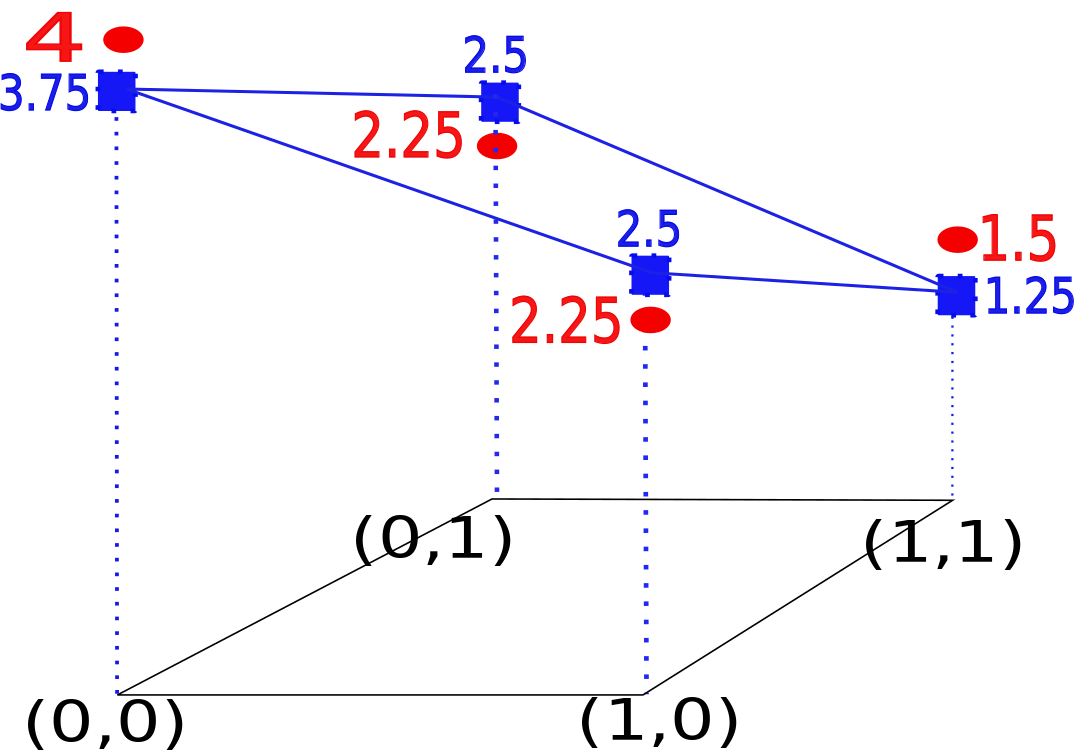
\includegraphics[width=2in,height=2in]{sec4fig.png}
	\caption{{\small The LSRM predicted sample sample rankings ($\hat{Y}=3.75-1.25U-1.25V$ (square vertices) have residual errors as the actual sample profile rankings (dots) do not belong to the plane of regression. }}	
	\label{sec4fig}
\end{figure}

 LSMR will not predict exact PAL rankings as the latter   are computed from the sample profile rankings (Table \ref{LSMR}).
 
 \begin{table}[!htpb]
 	\centering
 	\scriptsize
 	\begin{tabular}{c|cccc|c|c|c}
 		\multicolumn{2}{c}{} &\multicolumn{4}{c}{Respondent PAL Ranking}\\\hline
 		PAL & R 1&  R 2& R 3& R 4 &Sample PAL Rank&Predicted Sample Rank& $\mid$Residual Error$|$\\  \hline
 		$U=1$ &1.5&2&2&2&1.875&1.875&0\\
 		$U=0$&3.5&3&3&3&3.125&3.125&0 \\
 		$V=1$&3&2&2&2&1.875 &1.875&0 \\
 		$V=0$&4&4&4&4&3.125 &3.125&0\\\hline
 	\end{tabular}
 	\caption{{\small Predicted rankings for the sample outcomes in Table \ref{Tab1}.}}
 	\label{LSMR2}
 \end{table}

\subsection{Maximum Likelihood Estimation of PAL-ranking Intervals}
We will proceed to develop PR-ACBC methodology without assuming any knowledge of partworth utilitities.  Since computation of sample PAL rankings is easily computed from sample attribute rankings, we discuss how to obtain the population attribute rankings most likely to have given the observed sample attribute rankings.
\subsubsection{Known Population Size}
Let us assume our population has size $N=7$, and that our sample was a random selection of $n=4$ out of these 7. The number $N=7$ is for simplicity of illustrating the relevant cnmputations only, and could be any number $N>n=4$.  We will now use a multivariate hypergeometric distribution to obtain the maximum likelihood estimate (MLE) population profile rankings, meaning the population which was must likely to have yielded the observed sample profile rankings.  

Suppose in our sample with $n=4$,  three different profile rankings $O_1,O_2,O_3$ are observed, with ranking $O_2$ ocurring twice in the sample. We create what we shall call a \emph{factor table} to determine the MLE population (see Table \ref{FT}) 
\begin{table}[!htpb]
	\scriptsize
	\centering
	\begin{tabular}{r|ccc|c}\hline
		\multicolumn{5}{c}{Choose the $k=3$ largest factors $f_{ij}$ for a population size $N=n+k=n+3$.}\\ 
		+3& $f_{13}=4/3$ & $f_{23}=5/3$&$f_{33}=4/3$&\\
		+2& $f_{12}=3/2$ & $f_{22}=2$ &$f_{32}=3/2 $&\\
		+1& $f_{11}=2$  &$f_{21}=3$&$f_{31}=2 $ &\\\hline
		Number observed in sample:&$n_1=1$& $n_2=2$ & $n_3=1$ & Sample size: $n=4$\\\hline
		Ranking:&1=$O_1$&2=$O_2$&3=$O_3$
	\end{tabular}
	\caption{Probability factor table. The $k=3$ largest factors $f_{ij}=1+(n_i/j)$ are used to determine the MLE PRT for a population size $N=n+k=4+3=7$. }
	\label{FT}
\end{table}
{\flushleft  Let} $N_j$ denote the number of rankings $O_j$ in the PRT.  The number of factors $a_j$ chosen from column $j$ indicates that a  PRT with $N_j= n_j+a_j$ is a MLE.    In our case, the latter is not unique.  One choice of 3 largest factors is $f_{11}=2, f_{21}=3,f_{22}=2$ so that $a_1=1$, $a_2=2$ and $a_3=0$. A population $Y$ in which $N_1=n_1+a_1=2$ , $N_2=n_2+a_2=4$, and $N_3=n_3+a_3=1$ is a MLE. Another choice of 3 largest factors  is $f_{11}=2, f_{21}=3,f_{31}=1$ so that $a_1=1$, $a_2=1$ and $a_3=0$. Population $Z$ in which $N_1=n_1+a_1=2$ , $N_2=n_2+a_2=3$, and $N_3=n_3+a_3=2$ is also MLE. We can verify this is so by computing the respective probabilities $p_Y$ and $p_Z$ that our observed sample arises from erspective populations $Y$ and $Z$ :

\begin{equation}
p_Y=\frac{C(2,1)C(4,2)C(1,1)}{C(7,4)}=\frac{f_{11} \cdot f_{21}f_{22}}{C(7,4)}
\end{equation}
{\flushleft and }
\begin{equation}
p_Z=\frac{C(2,1)C(3,2)C(2,1)}{C(7,4)}=\frac{f_{11}\cdot f_{21}\cdot f_{31}}{C(7,4).}
\end{equation}
{\flushleft This} procedure generalizes to any number of rankings $m$ which appear in a sample of sample $n$ ( Oberhofer and Kaufman (1987)). Let $n=\sum_{j=1}^m n_j$ where $n_j$ is the number of ranking $j$ appearing in the sample.  Form the probability factor table with $f_{ij}=1+\frac{n_i}{j}$ ($i=1,...,r$, $j=1,...,m$ and $N=n+r$.)  Choose the $r$ largest factors in the latter table and let $a_j$ be the number of factors chosen in column $j$.  Then a population with a PRT such  $N_j=n_j+a_j$ ($j=1,...,m$) is a MLE. 
\subsubsection{Unknown Population Size}


Let us assume now that rather than having a specified size, the population size is an unknown value $N$.  In this case, we wish to determine the probability $p_i$  that a member of the population has ranking $O_i$.  As before, we assume that our sample is drawn randomly from the population. The probability $p$ that the observed sample consisting of one $O_1$, two $O_3$'s and one $O_9$ is

\begin{equation}
p=f(p_1,p_3,p_9)=\frac{4!}{1!2!1!}[p_1p_3^2p_9],
\end{equation}
\label{eq:1}
{\flushleft where} $g(p_1,p_3,p_9)=p_1+p_3+p_9=1$.
The values of $p_1^*,p_3^*,$ and $p_9^*$ which maximize $H(p_1,p_3,p_9)=\ln (f(p_1,p_3,p_9))$ (and hence also maximizes $p=f(p_1,p_3,p_9)$)  are obtained using Lagrange multipliers:
\begin{eqnarray*}
	\nabla H(p_1^*,p_3^*,p_9^*) & = & \lambda \nabla g
	(p_1^*,p_3^*,p_9^*),
\end{eqnarray*}
{\flushleft and therefore}
\begin{eqnarray*}
	\frac{1}{p_1^*} & = & \lambda\\
	\frac{2}{p_23^*} & = & \lambda\\
	\frac{1}{p_9^*} & = & \lambda.
\end{eqnarray*}
{\flushleft (The scalar quantity $\lambda$ is called a Lagrange multiplier.) Using} $p_1^*+p_3^*+p_9^*=1$ gives $\frac{1}{\lambda} + \frac{2}{\lambda}+\frac{1}{\lambda}=1$ and so $ \lambda = 4$.  Hence, the values $p_1^*=\frac{1}{4}, p32^*=\frac{1}{2}$, $p_9^*=\frac{1}{4}$ maximize the probability of the observed sample outcomes.  

In general, let $n_k$ be the number of sample outcomes $O_k$ ($k=1,2,...,K$) and let $p_k$ be the probability that a respondent in the population  has outcome $O_k$ $(k= 1, 2, ..., K)$.  The likelihood function $f(p_1, p_2, ..., p_K)$ giving the probability of observing the sample values $n_1, ..., n_{K}$ is given by

\begin{equation}
f(p_1, ...., p_K)= \frac{n!}{n_1!n_2!\cdot\cdot\cdot n_K!} \prod_{k=1}^K p_k^{n_k},
\end{equation}
\label{eq:4}

{\flushleft with} $\sum_{k=1}^{K}n_k=n$ and $\sum_{k=1}^{K}p_k=1$.
We seek to find the values $p_1^*, ..., p_{K}^*$ which maximize the likelihood function $f$, or equivalently, the log-likelihood function

\begin{equation}
H(p_1, ..., p_K)=\ln f = \ln(n!) - \sum_{k=1}^{K} n_k! +\sum_{k=1}^{K} n_k\ln(p_k),
\end{equation}
\label{eq:5}
{\flushleft subject} to the constraint $g(p_1, ..., p_{K})=p_1+p_2+...+p_K=1$.  Properties of gradients imply that the optimal values $p_i^*$ must satisfy

\begin{equation}
\nabla H(p_1^*, ..., p_K^*) = \lambda \nabla g(p_1^*, ..., p_{K}^*).
\end{equation}
\label{eq:6}
{\flushleft It} follows that for $k=1, ..., K$,

\begin{equation}
\frac{n_k}{p_k^*}=\lambda.
\end{equation}
\label{eq:7}
{\flushleft Hence,} $n=\sum_{k=1}^{K} n_k =  \lambda \sum_{k=1}^{K} p_k^* = \lambda$, and so the probabilities $p_k^* = \frac{n_k}{n}$ give the maximum likelihood of the observed sample outcomes $n_k$ ($k=1, 2, ..., K$).  For any sample of size $n$ and number $n_k$ of observed outcomes $O_k$ ($k=1, 2, ...K$), the maximum likelihood probabilities $p_k^*=\frac{n_k}{n}$
indicate that for a population of size $N$, the expected number $N_k$ of outcomes $O_k$ is given by $E(N_k)=p_k N.$  A maximum-likelihood population could be simulated by augmenting the observed $n$ sample outcomes, where the probability of outcome $O_k$ at each draw is given by $p_k$.   For a large number of such randomly constructed populations of size $N$, for each $k$ the average number of population outcomes $O_k$ is approximately $p_k N$.






\subsection{PAL Ranking Intervals}

Maximum likelihood  provides a point estimates into the population profile rankings and their corresponding PAL rankings.  Suppose a profile X in a sample of size $n$ has mean profile ranking $r_n(X)$.  It is easy to construct an interval which contains the mean ranking $\rho_N(X)$ for any population size $N>n$:

\begin{equation}
1+\frac{n}{N}(\rho_n(X)-1)\le \rho_N(X)  \le 4-\frac{n}{N}(4-\rho_n(X))
\label{eq6}
\end{equation}

{\flushleft This} interval containing $\rho_N(X) $ is obtained by either (i) assigning the  rank 1 to $X$ for all $N-n$ members of the population not in the sample (lower bound for $\rho_N(X)$); or (ii) assigning the rank 4 to $X$  for all $N-n$ non-sample population members (upper bound for $\rho_k(X)$). Let  $\lambda=\frac{N-n}{N}$ be the fraction of the population not included in the sample.  It is easy to show that
\begin{equation}
\rho_n(X)-\lambda(\rho_n(X)-1)\le \rho_N(X) \le \rho_n(X) + \lambda(4-\rho_n(X)).
\label{PRI}
\end{equation}

{\flushleft We} call (\ref{PRI}) the population profile ranking interval (PRI) for profile $X$.  The length of this interval is 
  $3\lambda$, where the 3 arises algebraically as the difference between  the extreme rankings 1 and 4.

\begin{figure}[!htpb]
\centering
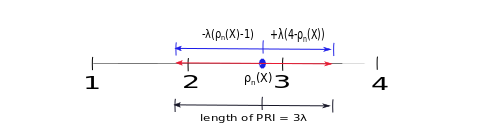
\includegraphics[width=6.5in, height=1.75in]{Confidence_Interval.png}
\caption{Given a profile $X$ and its sample ranking $\rho_n(X)$, the length of the population profile ranking interval (PRI) is determined by $\lambda=\frac{k-n}{k}$, the proportion of the population who have not taken the survey.}
\label{AL}
\end{figure}



The PRI can be used to quantify sample bias. Assume that, out of a total population $N=8$, two respondents have refused to take the survey, four have completed it, and the other two have not yet replied. In this case, the length of the PRI is  $\frac{3(8-4)}{8}=3/2$. If one of the non-respondents is convinced to participate, the interval length is reduced to $\frac{3(8-5)}{8}=\frac{9}{8}$, and if both non-respondents participate, then the interval is further reduced to $\frac{3(8-6)}{8}=\frac{3}{4}$. In other words, the two non-respondents  cause the length of the PRI interval to be twice as large, an important consideration in seeking to elicit survey response.


\subsubsection{Population Attribute Ranking Intervals}
In a similar way, if PAL $\chi$ has a sample ranking mean $\rho_n(\chi)$, it is easy to form  a \emph{PAL ranking interval} for any population $N>n$. For our toy survey,

\begin{equation}
r_n(\chi)+2(N-n)r_n(\chi)\le r_N(\chi) \le r_n(\chi)+8(N-n)r_n(\chi),
\end{equation}

{\flushleft which} is equivalent to  
\begin{equation}
r_n(X)-\lambda(r_n(X)-1)\le r_N(X) \le r_n(X) + \lambda(4-r_n(X)).
\label{ALRI}
\end{equation}
{\flushleft with} $\lambda=\frac{N-n}{N}$. Note that (\ref{PRI}) and (\ref{ALRI}) have the same form, so the length of both intervals is $3\lambda$.

\subsection{Multimensional Scaling}
One further type of analysis of PAL ranking data is a 2-dimensional geometric representation known as multidimensional scaling (MDS) (Alvo and Yu 2014). 
Fundamental to MDS is use of a distance measure $d(\mu,\nu)$ in which the more similar (resp. dissimilar) are a pair of rankings $\mu$ and $\nu$, the smaller (resp. larger).  A variety of distance measures have been used for MDS. For example, Hamming distance (from coding theory) is defined as
 
 \begin{equation}
 d_H{(\mu,\nu)}=t-\sum_{i=1}^t I(\mu(i)=\nu(i)).
 \end{equation}
 {\flushleft The} indicator function $I(\cdot)$ equals 1 if the statement inside parenthesis is true and 0 otherwise.  Hamming distance counts the number of positions where the permutations are different.
 
 
 Another example is Spearman distance, which is akin to usual Euclidean distance

\begin{equation}
d_S{()\mu,\nu)}=\frac{1}{2}\sum_{i=1}^t(\mu(i)-\nu(i))^2.
\end{equation}

{\flushleft Note} that Hamming distance formula satisfies the three required metric properties:

\begin{itemize}
	\item NON-NEGATIVITY $d_S(\mu,\nu)\ge 0$ for all $\mu$, $\nu$, with equality holding if and only if $\mu=\nu$;
	\item SYMMETRY $d_S(\mu,\nu)=d_S(\nu,\mu)$ 
	\item TRIANGLE INEQUALITY $d(\mu,\nu)+d(\nu,\sigma)\ge d(\mu,\sigma)$.
\end{itemize}
{\flushleft Spearman distance}, however, only satisfies the first two metric properties (Alvo and Yu ).

 For PR-ACBC, let $(i,j)$ denote level $j$ of attribute $i$,  and let $f(i,j)$ be the average rank of level $(i,j)$ in an individual respondent's profile ranking. For example, for the profile ranking BACD, $f(1,1)=(1+2)/2=1.5$ since B=10 is ranked first and A=11 is ranked second; $f(20)=(2+4)/2=3$ since B=10 is ranked second and $D=00$ is ranked 4th.

 For our toy survey, each respondent $X$ will have four average profile level rankings $f_X(1,1), f_X(1,0), f_X(2,1), f_X(2,0)$.  Given 2 respondents $X$ and $Y$, we consider the squared Euclidean distance between their PAL rankings defined as
\begin{equation}
d_S(X,Y)=\sum_{i,j} [f_X(i,j)-f_Y(i,j)]^2.
\label{Spea}
\end{equation}

{\flushleft This} distance measure can be used for an ACBC survey with any number of attributes and levels.


Once a distance measure is defined, a 2-dimensional MDS is such that rankings are represented by points in an xy Cartesian coordinate system, and the Euclidean distance between these points reflects the relative distances between rankings.   
Note that in this MDS, respondents R2 and R4 coincide since they have the same ranking (ACBD).   

\begin{figure}[!htpb]
	\centering
	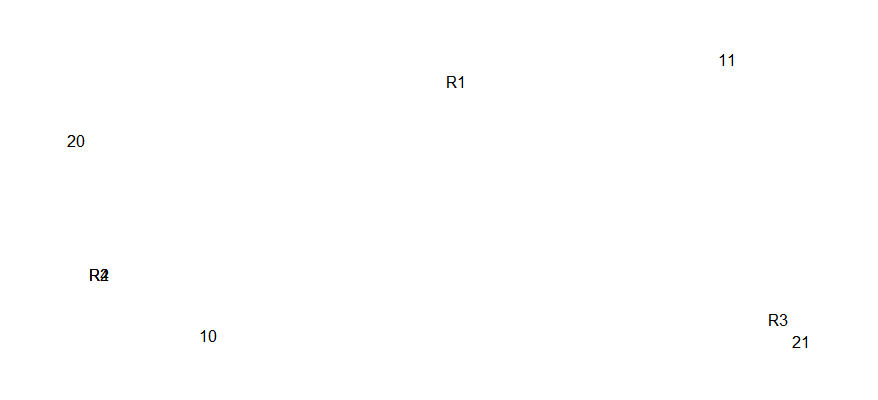
\includegraphics[width=6.5in, height=1.75in]{MDS1.png}
	\caption{Example of an MDS using the distance function defined in (\ref{Spea}) . In this case the sample profile rankings are ABCD, ACBD (twice), and BCAD}
	\label{AL}
\end{figure}




\section{ACBC Survey of Humanitarian Disaster Relief Organizations}

PR-based ACBC methodology for analyzing small populations has many possible applications. One application involves  a study of a small population ($N\approx 50$) of international, Christian faith-based disaster relief organizations headquartered in the U.S. as well as their non faith-based counterparts, will all organizations belonging to the National VOAD.




{\bf TASK 2: MAKE A TABLE OF THE N-VOAD ORGANIZATIONS CONTACTED FOR THE SURVEY} 

In disaster relief, effectiveness of a response may depend on the quality of collaboration between organizations with a broad diversity of religious and ideological perspectives. For effective coordination of relief, it is important that humanitarian organizations understand the unique traits and characteristics that shape their disaster response decisions. Through comparison of these factors, it is possible to design optimal partnerships and joint endeavors between organizations that may fulfill distinct, yet complimentary, humanitarian roles. Our research focuses on a few key attributes affecting our population group's decision whether or not to respond to an international humanitarian disaster.


To this end, we designed an ACBC survey that creates disaster profiles with attributes and levels for this survey are displayed in Figure \ref{AL}. Different disaster scenarios are paired off  in the choice task (single elimination tournament) stage, beginning with 16 profiles close to the Build-Your-Own (BYO) or ideal scenario. The tournament data is the basis for profile ranking. The survey was deployed and tournament data collected using Sawtooth's Lighthouse platform.



\begin{figure}[!htpb]
\centering
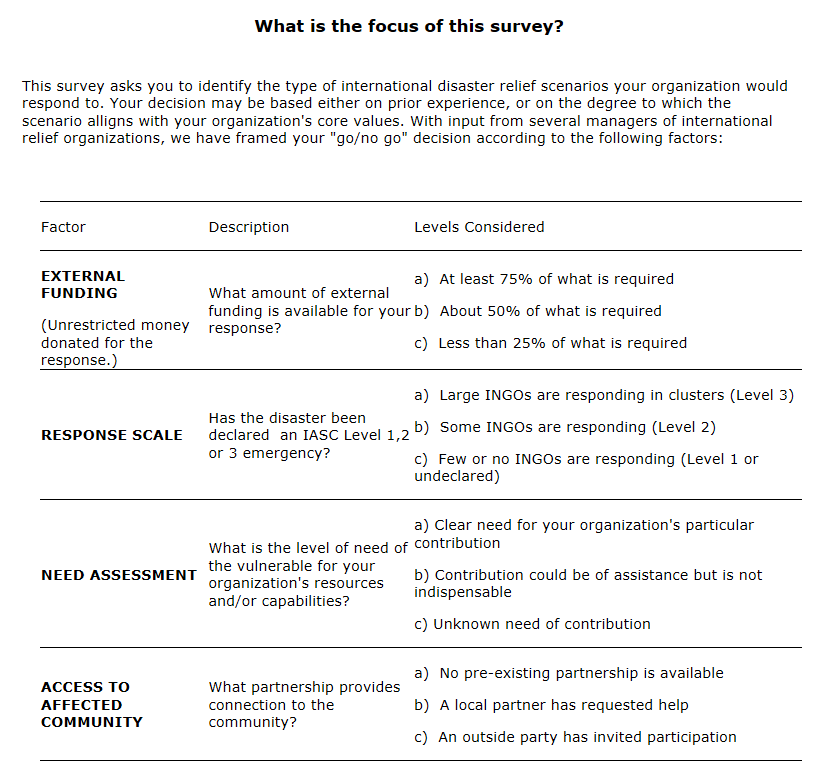
\includegraphics[width=5.75in, height=7in]{AttributeLevels.png}
\caption{{\small An ACBC survey with 4 attributes consisting of 3 levels each. }}
\label{AL}
\end{figure}


\subsection{Survey Data}

As shown in Figure 4, our humanitarian survey consists of four attributes, each with three levels. Thus, the number of possible profiles is $3^4=81$. These are identified by four digit numbers $X=x_1x_2x_3x_4$ where profile $X$ has level $x_1$ for the first attribute, level $x_2$ for the second attribute, level $x_3$ for the third attribute, and level $x_4$ for the fourth attribute. In the tournament stage of the competition, there are four rounds, in which sixteen profiles face off against each other in head to head match-ups, much like the FIFA World Cup Round of 16. The competing profiles are selected from the 81 possible profiles based on the respondent's BYO preferences. We assign a ranking of 1 to the tournament winner, 2 to the runner up, 3 to the semifinal losers, 4 to the quarterfinal losers, 5 to the profiles that are eliminated in the first round, and 6 to those that do not appear in the tournament. The survey was first deployed to FBOs, with the results shown in Table \ref{Tab13}. 



\begin{table}[!htpb]
\scriptsize
\centering
\begin{tabular}{c|ccccc|ccccc|ccc|c}
Profile& 1 & 2 & 3 & 4 & 5 & 6&7&8&9&10&11&12&13&PR\\\hline
1212& 2&	3&	7&	3&	7&	7&	1&	7&	7&	7&	4&	1&	7&	4.846\\
1112&7	&1	&7	&7	&1	&2	&7	&5	&7	&3	&7	&7	&4	&5.000\\
1312&7	&7	&7	&7	&5	&5	&7	&1	&1	&1	&7	&7	&3	&5.000\\
3212&7	&7	&7	&5	&5	&1	&2	&7	&4	&7	&7	&7	&1	&5.154\\
1122&1	&7	&7	&4	&7	&7	&5	&7	&4	&7	&3	&3	&7	&5.308\\
2212&7	&5	&5	&7	&7	&7	&7	&2	&7	&4	&2	&2	&7	&5.308\\
1222&7	&7	&4	&7	&4	&5	&7	&4	&3	&2	&7	&7	&7	&5.462\\
1232&5	&7	&7	&5	&5	&5	&4	&5	&7	&5	&7	&7	&2	&5.462\\
2312&7	&7	&7	&1	&5	&3	&4	&7	&2	&7	&7	&7	&7	&5.462\\
2112&3	&7	&7	&4	&5	&4	&3	&7	&7	&7	&7	&7	&5	&5.615\\\hline
\end{tabular}
\caption{{\small Top 10 ranked profiles for FBOs ($n=13,N=50$) }   }
\label{Tab13}
\end{table}

{\bf TASK 3 ADD SIMILAR TABLE FOR NON FBO DATA}


\subsection{Survey Analysis}
{\bf TASK 4 MLE}



{\bf TASK 5 Population Profile Rank Intervals}



{\bf Task 6 MDS of Profile Attributes }


\subsection{Comparison with Part-worth Utilities}

{\bf Task 7 Choice task prediction accuracy}

{\bf Task 8 Attribute Importances}




\section{Conclusion}
Unlike conjoint analysis of survey data where the target populations are large and more suitable for conventional statistical tools, we have introduced a simple, intuitive approach to a small population's profile rankings based on sample data. 

{\bf Task 9 COMPLETE CONCLUSION}

Major areas open to further research include analysis of  different ranking systems for various types of choice tournaments and application of PR ACBC methodology to other small population studies.



\subsection*{Acknowledgements}

Ming-Hsuan Chuang,
Daniel Daum, Michaela Flitsch, Erica Gralla, Jarrod Goenzel, Timotius Kartawijaya, Zoe Kallus, Courtney Linscott, Sara Magnuson, Mark Nussbaum, Zach Oslund, Matthew Rueger,, Nick Varberg, Mike Veatch, Joyce Yan   

\section*{References}
\begin{list}{}{\itemindent=-2em}
\small
\item Alvo, M., and Yu, P.L.H. 2014. \emph{Statistical Methods for Ranking Data}. Springer.

\item Gralla, E., Goentzel, J., and Fine G. 2014. Assessing trade-offs among multiple objectives for humanitarian aid delivery using expert preferences.
\emph{Production and Operations Management}, Springer-Verlag Berlin 23(6), 978-989.

\item Oberhofer, W. and Kaufman, H.1987.  Maximum Likelihood Estimation of a Multivariate Hypergeometric Distribution. \emph{Sankhya: The Indian Journal of Statistics, Series B (1960-2002)}, Indian Statistical Institute, 49(2), 188-191. 

\item Orme, B.K., and Chrzan, K. 2017. \emph{Becoming an Expert in Conjoint Analysis: Choice Modeling for Pros.} Sawtooth Software.

\item Rao, V. R. 2014. \emph{Applied Conjoint Analysis}. Springer.

\item  Stewart, J. 2016.  \emph{Calculus, Early Transcendentals (8E)}. Cengage Learning.

\item Rossi, P., Allenby, G. and McCulloch R. 2005. \emph{Baysian Statistics and Marketing.} John Wiley \& Sons, Ltd.


\end{list}
\end{document}
